\documentclass[11pt,a4paper]{article}
\usepackage[utf8]{inputenc}
\usepackage[french]{babel}
\usepackage{amsmath}
\usepackage{amsthm}
\usepackage{amsfonts}
\usepackage{amssymb}
\usepackage{graphicx}
\usepackage[font=small]{caption}
\usepackage{wrapfig}
\usepackage{subfig}
\usepackage[a4paper,width=140mm,top=25mm,bottom=25mm]{geometry}
\author{}
\title{\textbf{Symétries de 4S}}
\date{}





% packages for layout
\usepackage{fancyhdr}
\pagestyle{fancy}
\fancyhf{}
\fancyhead[L]{\textit{\nouppercase{\leftmark}}}
\fancyhead[R]{\thepage}

\renewcommand{\headrulewidth}{0.5pt}


%roman enumeration
\renewcommand\labelenumi{(\roman{enumi})}
\renewcommand\theenumi\labelenumi

% font
%\usepackage{pxfonts}

% bibliography
\usepackage[style=numeric, backend = biber]{biblatex}
\bibliography{/Users/philipp/Documents/Studium/Stage/tex/stage.bib}

% environments
% theorem
\theoremstyle{plain}
\newtheorem{theorem}{Théorème}
% corollary
\theoremstyle{plain}
\newtheorem{corollary}{Corollaire}
% lemma
\theoremstyle{plain}
\newtheorem{lemma}{Lemme}
% remark
\theoremstyle{definition}
\newtheorem*{remark}{Remarque}
% definition
\theoremstyle{definition}
\newtheorem{definition}{Définition}
% example
\theoremstyle{definition}
\newtheorem{example}{Example}
% proposition
\theoremstyle{plain}
\newtheorem{proposition}{Proposition}

% additional packages
\usepackage{appendix}
\usepackage{amsmath}
\usepackage{amsfonts}
\usepackage{amssymb}
\usepackage{amsthm}
\usepackage{booktabs}

\newcommand{\N}{\mathbb{N}}
\newcommand{\M}{\mathcal{M}}
\newcommand{\R}{\mathbb{R}}
\DeclareMathOperator{\asym}{Asym}
\DeclareMathOperator{\id}{id}
\newcommand{\h}{\mathcal{H}}
\newcommand{\so}{\mathfrak{so}}

\begin{document}
\linespread{1.05}
\maketitle

\section{Préliminaires}
L'espace des états de 4S est donné par $\mathcal{M} = (\sqrt{3/2}, + \infty)^4$, tandis que l'espace des positions est donné par $\mathcal{P} = \R^3 \times SO(3)$. Ici, on fait l'identification
\begin{align*}
	SO(3) = \{R \in O(3) \mid \det(R) = 1\} \subset M_{3 \times 3}(\R).
\end{align*}
On notera $I$ la matrice d'identité de $M_{3 \times 3}(\R)$ et les rotations élémentaires autour des axes des coordonnées $R_{z}(\theta)$ et similaire pour $x$ et $y$. On caractérise l'orientation du nageur par la direction du quatrième bras et l'angle entre le premier bras et l'axe $x$. On fixe la convention que l'orientation correspondante à l'identité et celle où le quatrième bras est aligné à l'axe $z$ et l'angle entre le premier bras et l'axe $x$ vaut zéro.

Nous avons vu dans \textit{Optimally Swimming Stokesian Robots} que le problème de contrôle associé au nageur 4S s'écrit 
\begin{align}
\label{eq:control_problem}
\begin{cases}
\dot{p} = \sum_{i = 1}^{4} \mathbf{F}_i(R, \xi)\dot{\xi}_i\\
p(0) = p_0,
\end{cases}
\end{align}
où les $\mathbf{F}_i$ sont des champs de vecteurs sur $T \mathcal{P}$.

\begin{figure}[h]
	\centering
		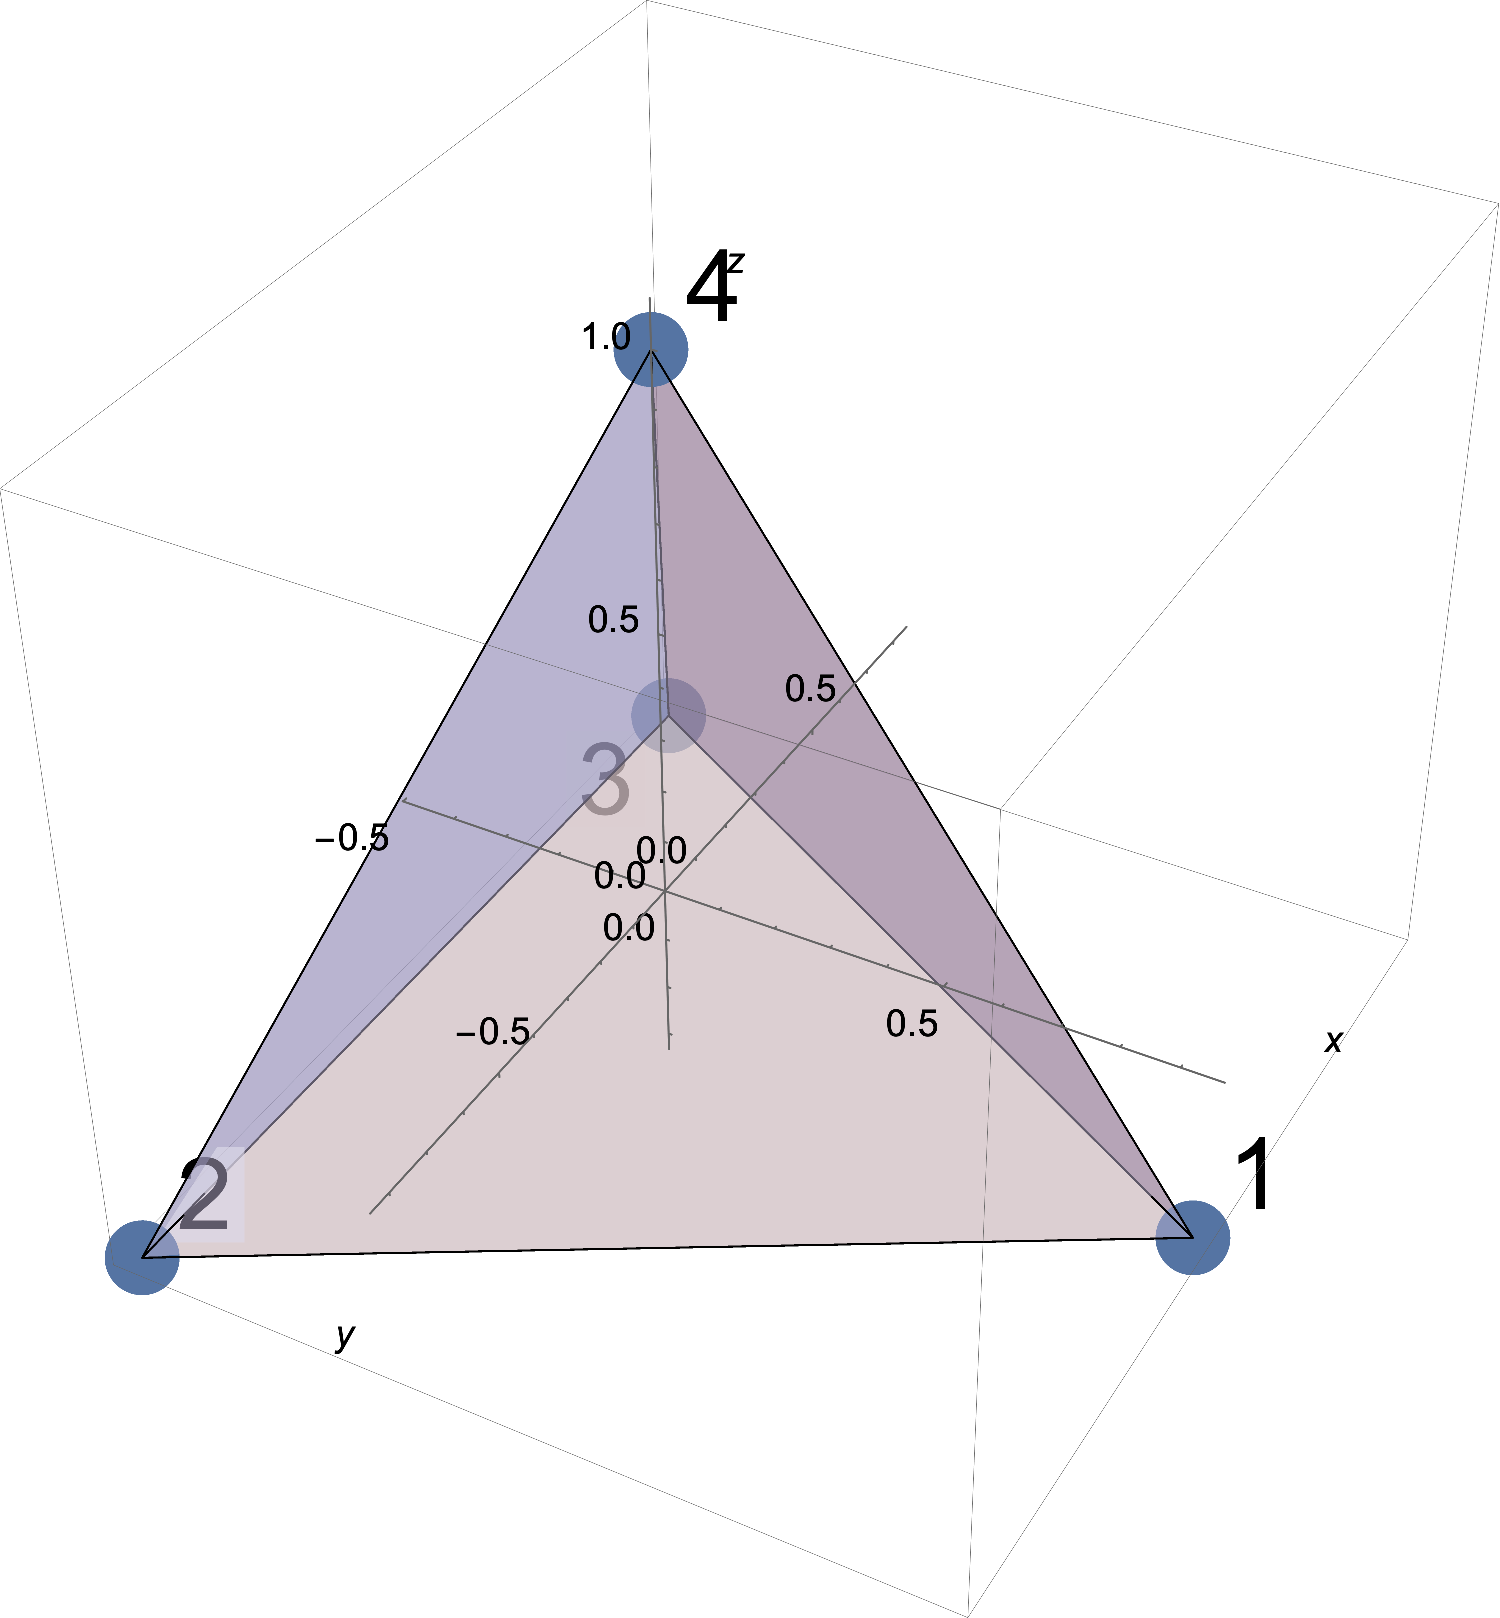
\includegraphics[scale = 0.5]{/Users/philipp/Documents/Studium/Stage/mathematica/id_pos.png}
	\caption{La position du nageur 4S correspondante à l'identité}
	\label{fig:globalintensity_china}
\end{figure}


\section{Symétrie rotationnelle}

\begin{lemma}
A un point $R \in SO(3)$ l'espace tangent est donné par
\begin{align*}
	R^* \asym_3(\R) = \{RA \mid A \in \asym_3(\R)\},
\end{align*}
où $\asym_3(\R)$ désigne les matrices réelles antisymétriques de taille 3.
\end{lemma}

\begin{proof}
On remarque d'abord qu'il suffit de calculer l'espace tangent à l'identité car $SO(3)$ est un groupe de Lie et donc $SO(3)$ agit sur soi-même par difféomorphismes. En effet, si on connaît l'espace tangent à l'identité, l'espace tangent à un point arbitraire $R \in SO(3)$ est donné par le tire-en-arrière $T_{R}SO(3) = R^{*}T_{I}SO(3)$. De plus, $SO(3)$ est la composante connexe de l'identité de $O(3)$ (par continuité de la déterminante). Par conséquent, nous avons $T_{I}SO(3) = T_{I}O(3)$. Or, d'après le théorème du rang constant, $O(3)$ est défini par $O(3) = \Phi^{-1}(I)$, où $\Phi: GL(\R,3) \to M_{3 \times 3}(R)$ est donné par $\Phi(A) = A^T A$. Pour $Q \in GL(\R,3)$, la différentielle $d_{Q} \Phi: T_QO(3) \to T_{Q^TQ}M_{3 \times 3}(\R)$ est donnée par $R \mapsto RQ + QR^T$, en particulier à l'identité nous avons $d_I \Phi(R) = R + R^T$. Il suit d'un corollaire du théorème du rang constant que
\begin{align*}
	T_I O(3) = \ker d_I \Phi = \{R \in M_{3 \times 3}(\R) \mid R + R^T = 0\} = \asym_3(\R).
\end{align*}
\end{proof}

Avec ce lemme, on trouve que pour tout $p = (\mathbf{c} ,R) \in \mathcal{P}$ on a $T_p \mathcal{P} \simeq \R^3 \times R^{*}\asym_3(\R)$. En particulier, on peut écrire le système (\ref{eq:control_problem}) sous la forme 
\begin{align*}
\dot{p} = F(R, \xi) \dot{\xi} = (F_c(R, \xi) \dot{\xi}, F_\theta(R, \xi) \dot{\xi}),
\end{align*}
où  $F_c(R, \xi) \in M_{3 \times 4}(\R)$ et $F_\theta(R, \xi) \in \mathcal{L}(\R^4, R^* \asym_3(\R))$.

Soit maintenant $p_0 = (c_0, R_0)$ une position initiale et $\xi: I \subset \R \to \M$ une courbe de contrôle avec $I$ un voisinage de zéro et $\xi_0 := \xi(0)$. Soit $\gamma(p_0, \xi) = (\gamma_c(p_0, \xi), \gamma_\theta(p_0, \xi))$ la solution associée au système (\ref{eq:control_problem}) avec condition initiale $p(0) = p_0$. Il suit de l'invariance rotationnelle des équations de Stokes que pour tout $R\in SO(3)$
\begin{align}
\label{eq:spatial_rot_inv}
	\gamma_c(c_0, R R_0, \xi)(t) &= R \gamma_c(c_0, R_0, \xi)(t) + (I - R)c_0\\
\label{eq:ang_rot_inv}
	\gamma_\theta(c_0, R R_0, \xi)(t) &= R \gamma_{\theta}(c_0,R_0, \xi)(t)
\end{align}


\begin{proposition}
\label{prop:rot_inv}
Soit $\xi_0 := \xi(0) \in \M$ l'état initial des paramètres de contrôle et $T_{\xi} \M$ l'espace tangent de $\M$ à $\xi$. Si le système de contrôle (\ref{eq:control_problem}) est invariant sous rotations et si $T_{\xi} \M \simeq \R^4$, alors
\begin{align*}
	F(R, \xi) =  (R F_{c}(\xi), R F_{\theta}(\xi) )& & \text{ avec } & & F_{c}(\xi):= F_{c}(I, \xi), F_{\theta}(\xi) := F_{\theta}(I, \xi)
\end{align*}
pour tout $(R, \xi) \in SO(3) \times \M$.
\end{proposition}

\begin{proof}
Par définition du système (\ref{eq:control_problem}) on a
\begin{align*}
	\dot{\gamma}_{c}(c_0, R R_0, \xi)(t) &= F_{c} \left ( \gamma_{\theta}(c_0, R R_0, \xi), \xi \right ) \dot{\xi}(t),\\
	\dot{\gamma}_{\theta}(c_0, R R_0, \xi)(t) &= F_{\theta} \left ( \gamma_{\theta}(c_0, R R_0, \xi), \xi\right ) \dot{\xi}(t)
\end{align*}
Par (\ref{eq:spatial_rot_inv}) et (\ref{eq:ang_rot_inv}), on a également par définition du système
\begin{align*}
	\dot{\gamma}_{c}(c_0, R R_0, \xi)(t) &= R F_{c}(\gamma_{\theta}(c_0,R_0,  \xi), \xi) \dot{\xi}(t)\\
	\dot{\gamma}_{\theta}(c_0, R R_0, \xi)(t) &= R F_{\theta}(\gamma_{\theta}(c_0, R_0, \xi), \xi) \dot{\xi}(t)
\end{align*}
\
Ainsi, on trouve pour tout $R \in SO(3)$
\begin{align*}
	F_{c} \left ( \gamma_{\theta}(c_0, R R_0, \xi),  \xi \right ) \dot{\xi} &= R F_{c}(\gamma_{\theta}(c_0, R_0, \xi), \xi) \dot{\xi}\\
	F_{\theta} \left ( \gamma_{\theta}(c_0, R R_0, \xi), \xi\right ) \dot{\xi} &= R F_{\theta}(\gamma_{\theta}(c_0, R_0, \xi), \xi) \dot{\xi},
\end{align*}
Vu que $T_{\xi}\M \simeq \R^4$, évaluation à $t = 0$ de cette dernière expression fournit $F_{c}(R \, R_0, \xi_0) = RF_{c}(R_0, \xi_0)$ et $F_{\theta}(R \, R_0, \xi_0) = R F_{\theta}(R_{0}, \xi_0)$. Finalement, si on définit $R_0 = I$, on obtient le résultat souhaité.
\end{proof}

\section{Permutation des bras}
D'abord, on définit les matrices de permutations suivantes:
\begin{align*}
	L = (e_2 \mid e_1 \mid e_3 \mid e_4) & & M = (e_1 \mid e_3 \mid e_2 \mid e_4) & &
	N = (e_1 \mid e_2 \mid e_4 \mid e_3)
\end{align*}
où si on les applique à $\M$, les matrices $L, M, N$ et $O$ correspondent aux permutations des bras $||1\leftrightsquigarrow ||2, ||2\leftrightsquigarrow ||3, ||$ et 
$3\leftrightsquigarrow ||4$ respectivement. On notera $S_{xy}(\phi)$ la réflexion à un plan orthogonal au plan $xy$ faisant un angle $\phi$ avec l'axe $x$. On notera $S_{yz}(\phi)$ l'analogue pour le plan $yz$. De plus, on remarque pour la suite que l'angle entre deux bras d'un tétraèdre, \emph{l'angle du tétraèdre}, est donné par
\begin{align*}
	\alpha_{tet} = \arccos(-1/3).
\end{align*}
Comme pour l'invariance rotationnelle on traitera la partie spatiale et la partie angulaire séparément.

\subsection{Symétrie spatiale}
Pour chaque permutation on fixe une orientation de référence $R_L, R_M$ et $R_N$ respectivement de sorte que les deux bras en question soient symétrique par rapport au plan $yz$. Pour alléger la notation, on écrit $S := S_{xy}(\tfrac{\pi}{2})$. De plus, on pose  $R_{L} = R_{z}(-\pi/6), R_{M} = R_{z}(\pi/2)$ et $R_{N} = R_{z}(-\pi/6)R_{y}(-\alpha_{tet})$. Finalement, on fixe pour toutes les trois permutations une position spatiale de référence $c_{\mathrm{ref}} \in \R^3$. Soient alors $\gamma(c_{\mathrm{ref}}, R_L, L\xi), \gamma(c_{\mathrm{ref}}, R_M, M\xi)$ et $\gamma(c_{\mathrm{ref}}, R_N, N\xi)$ des solutions du système de contrôle.
Ainsixx, on trouve grâce à l'invariance sous changement de point d'observations des équations de Stokes, i.e. en regardant les solutions dans un miroir, les relations
\begin{equation}
\label{eq:spat_perm_inv}
\begin{aligned}
		\gamma_c(c_{\mathrm{ref}}, R_L, L \xi) &= S\gamma_{c}(S c_{\mathrm{ref}}, R_L, \xi)\\
		\gamma_c(c_{\mathrm{ref}}, R_M, M \xi) &= S\gamma_{c}(Sc_{\mathrm{ref}}, R_M, \xi) \\
		\gamma_c(c_{\mathrm{ref}}, R_N, N \xi) &= S \gamma_{c}(Sc_{\mathrm{ref}}, R_N, \xi).
\end{aligned}
\end{equation}




Soit $p_0 = (c_o, R_0) \in \mathcal{P}$ une position initiale et $\gamma_{c}(c_0, R_0, L \xi)$ la partie spatiale de la solution du problème de contrôle. Pour tout $R \in SO(3)$, on a par (\ref{eq:spatial_rot_inv})
\begin{align*}
	\gamma_{c}(c_0, R_0, L \xi) = R^{-1} \gamma_{c}(c_0, R R_0, L \xi) - (R^{-1} - I) c_0.
\end{align*}
Soit $R_1 := R_{L}R_0^{-1}$. Par la condition (\ref{eq:spat_perm_inv}), on a
\begin{align*}
	\gamma_{c}(c_0, R_0, L \xi)(t) = R_{1}^{-1} S \gamma_c (Sc_0, R_{L}, \xi)(t) - (R^{-1}_1 - I) c_0.
\end{align*}
Ainsi, on trouve par définition du système et avec la proposition \ref{prop:rot_inv}
\begin{align*}
	\dot{\gamma}_c (c_0, R_0, \xi)(t)
	 &= \gamma_{\theta}(c_0, R_0, \xi)(t) F_c(L \xi) L \dot{\xi}(t)\\
	 &= R_{1}^{-1} S \gamma_{\theta}(Sc_0, R_{L}, \xi)(t) F_{c}(\xi) \dot{\xi}(t).
\end{align*}
Évaluation à $t = 0$ et le fait que $T_{\xi}\M \simeq \R^4$ pour tout $\xi \in \M$ fournissent 
\begin{align*}
	R_0 F_c(L \xi_0) L = R_{1}^{-1} S R_{L} F_c(\xi_0).
\end{align*}
En posant $S_L := R_{L}^{-1} S R_{L}$, on trouve alors $F_c(L \xi) = S_L F_c(\xi) L$ pour tout $\xi \in \M$. En particulier, ce calcul fonctionne de même pour les autres permutations et en posant
\begin{align*}
	S_{M} := R_{M}^{-1} S R_{M} & & S_{N} := R_{N}^{-1} S R_{N}
\end{align*}
nous avons alors démontré le résultat suivant.

\begin{proposition}
\label{prop:spat_perm_inv}
Pour toute courbe de contrôle $\xi$, l'application $F_c$ satisfait
\begin{align*}
	F_c(L \xi) = S_L F_c(\xi) L & &F_c(M \xi) = S_M F_c(\xi) M & &F_c(N \xi) = S_N F_c(\xi) N.
\end{align*}
\end{proposition}

\subsection{Symétrie angulaire}
On commence par quelques observations concernant la réflexion d'une rotation à un plan. Jusque là, nous avons identifié $SO(3)$ aux matrices orthogonales de déterminante 1. Or, le théorème d'Euler dit que pour toute rotation dans $SO(3)$ il existe une axe de rotation $\mathbf{u} \in S^2$ de sorte que l'on puisse la représenter par le vecteur d'Euler $\mathbf{\omega} = \theta \mathbf{u}$, où $\theta$ est l'angle de rotation. Le lien entre ces deux représentations est donné par l'exponentielle matricielle que l'on explicitera dans ce qui suit. On se rappelle que
\begin{align*}
	\so(3) = T_{I}SO(3) = \asym_3(\R).
\end{align*}
De plus, on notera $R_{x}(\theta), R_{y}(\theta)$ et $R_{z}(\theta)$ les rotations élémentaires autour des axes $x,y$ et $z$, respectivement. On voit facilement que $\dim \asym_3(\R) = 3$ et on trouve que les matrices
\begin{align*}
	&L_1 = \frac{d}{d\theta}R_x(\theta)_{\mid \theta =0} = \left(\begin{array}{ccc}
	0 & 0 & 0 \\ 
	0 & 0 & -1 \\ 
	0 & 1 & 0
	\end{array}  \right ),\\
	&L_2 = \frac{d}{d\theta}R_y(\theta)_{\mid \theta =0} = \left (\begin{array}{ccc}
	0 & 0 & 1 \\ 
	0 & 0 & 0 \\ 
	-1 & 0 & 0
	\end{array}  \right ),\\
	&L_3 = \frac{d}{d\theta}R_z(\theta)_{\mid \theta =0} = \left (\begin{array}{ccc}
	0 & -1 & 0 \\ 
	1 & 0 & 0 \\ 
	0 & 0 & 0
	\end{array}  \right ),
\end{align*}
forment une base de $\so(3)$ que l'on notera $\mathcal{L}$. Pour $A \in \so(3)$ on obtient avec les propriétés de l'exponentielle matricielle que
\begin{align*}
	(e^{A})^T e^{A} = e^{A^T} e^{A} = e^{-A} e^{A} = e^{I} = I.
\end{align*}
Donc, cette application est bien-définie et en particulier on a $R_z(\theta) = e^{\theta L_z}$ et similaire pour les autres rotations similaires. On remarque que pour tout $A \in \so(3)$ et $Q \in SO(3)$ on a $QAQ^T \in \so(3)$. Soit maintenant $R \in SO(3)$ quelconque. On trouve toujours un $Q \in SO(3)$ de sorte que
\begin{align*}
	R = Q R_{z}(\theta) Q^T = Q e^{\theta L_z} Q^{T} = e^{\theta QL_zQ^{T}} = e^{\theta \mathbf{u} \cdot \mathbf{L}},
\end{align*}
avec $\mathbf{L} = (L_x, L_y, L_z)^T$ où on permet un petit abus de notation et $\mathbf{u} \in S^2$ car $Q$ est une application orthogonale. Ceci montre bien que $\exp: \so(3) \to SO(3)$ est surjectif. Réciproquement, le calcul direct montre que pour une axe de rotation $\mathbf{u} \in S^2$ et un angle de rotation $\theta \in \R$ la matrice $R = \exp(\theta \mathbf{u} \cdot \mathbf{L})$ est bien la matrice de rotation associée.


Soit $S$ une réflexion à un plan dans $\R^3$ et $R \in SO(3)$ l'orientation d'un corps rigide dans $\R^3$ avec vecteur d'Euler $\omega$ associé. On notera $\tilde{R} \in SO(3)$ l'orientation de l'image miroir du corps rigide avec vecteur d'Euler $\tilde{\omega}$. On s'aperçoit que $\tilde{\omega} = -S \omega$, i.e. l'axe de rotation est reflétée et au même temps le sens de rotation est inversé pour les rotations parallèles au plan de réflexion. Un petit calcul montre que
\begin{align}
\label{eq:rep_ref}
\tilde{\omega} \cdot \mathbf{L} = S(\omega \cdot \mathbf{L})S,
\end{align}
dont il suit que
\begin{align}
	\tilde{R} = \exp(\tilde{\omega} \cdot \mathbf{L}) = \exp(S(\omega \cdot \mathbf{L}) S) = S R S.
\end{align}

Maintenant, on se donne une orientation de référence $R_{\mathrm{ref}} := R_z(-\tfrac{\pi}{6})$ ainsi que les réflexions $T_L := S_{xy}(\tfrac{\pi}{2}), T_{M} := S_{xy}(\tfrac{5\pi}{6})$ et $T_{N} := S_{yz}((\pi - \alpha_{tet})/2)$. De nouveau par l'invariance sous changement de point de vue des équations de Stokes justifient les relations suivantes, où on a directement compensé pour la position initiale.
\begin{equation}
\label{eq:ang_perm_inv}
\begin{aligned}
	\gamma_{\theta}(c_{\mathrm{ref}}, R_{\mathrm{ref}}, L \xi) &= R_{\mathrm{ref}} T_{L} R_{\mathrm{ref}}^{-1} \gamma_{\theta}(T_{L} c_{\mathrm{ref}}, R_{\mathrm{ref}}, \xi) T_{L}\\
	\gamma_{\theta}(c_{\mathrm{ref}}, R_{\mathrm{ref}}, M \xi) &= R_{\mathrm{ref}} T_{M} R_{\mathrm{ref}}^{-1} \gamma_{\theta}(T_{M}c_{\mathrm{ref}}, R_{\mathrm{ref}}, \xi) T_{M}\\
	\gamma_{\theta}(c_{\mathrm{ref}}, R_{\mathrm{ref}}, N \xi) &= R_{\mathrm{ref}} T_{N} R_{\mathrm{ref}}^{-1} \gamma_{\theta}(T_{N}c_{\mathrm{ref}}, R_{\mathrm{ref}}, \xi) T_{N}.
\end{aligned}
\end{equation}
Soit $p_0  = (c_0, R_0) \in \mathcal{P}$ une position initiale. Alors, nous avons par (\ref{eq:ang_rot_inv}) pour tout $R \in SO(3)$
\begin{align*}
	\gamma_{\theta}(c_0, R_0, L \xi) = R^{-1}\gamma_{\theta}(c_0, R R_0, L\xi).
\end{align*}
En particulier, pour $R_1 := R_{\mathrm{ref}} R_{0}^{-1}$ on obtient avec la condition (\ref{eq:ang_perm_inv})
\begin{equation}
\begin{aligned}
	\gamma_{\theta}(c_0, R_0, L \xi) &= R_{1}^{-1} \gamma_{\theta}(c_0, R_{\mathrm{ref}}, L \xi)\\
	 &= R_{1}^{-1} R_\mathrm{ref} T_{L} R_{\mathrm{ref}}^{-1}\gamma_{\theta}(T_{L}c_0, R_{\mathrm{ref}}, \xi) T_{L}.
\end{aligned}
\end{equation}
Par définition du système et en utilisant la proposition \ref{prop:rot_inv}, on obtient à $t = 0$
\begin{align}
	F_{\theta}(L \xi_0) L \dot{\xi}(0) = T_{L} F_{\theta}(\xi_0) \dot{\xi}(0) T_{L}.
\end{align}

On continue par représenter $F_{\theta}(\xi_0) \in \mathcal{L}(\R^4, \asym_3(\R))$ par une matrice $[F_{\theta}(\xi_0)]_{\mathcal{E}}^{\mathcal{L}} \in M_{3 \times 4}(\R)$ par rapport aux bases $\mathcal{L}$ et $\mathcal{E} = (e_1, e_2, e_3,e_4)$. En particulier, le calcul de (\ref{eq:rep_ref}) montre que la la matrice représentant l'application linéaire $A \in \asym_3(\R) \mapsto T_{L} A T_{L} \in \asym_3(\R)$ est donnée par $-T_{L}$ dans la base $\mathcal{L}$. Donc, nous avons par rapport aux bases $\mathcal{E}$ et $\mathcal{L}$
\begin{align*}
	&[F_{\theta}(L \xi_0) L \dot{\xi}(0)]_{\mathcal{E}}^{\mathcal{L}} = [F_{\theta}(L \xi_0)]_{\mathcal{E}}^{\mathcal{L}} L [\dot{\xi}(0)]_{\mathcal{E}},\\
	&[T_L F_{\theta}(\xi_0)\dot{\xi}(0)T_L]_{\mathcal{L}} = -T_L[F_{\theta}(\xi_0) \dot{\xi}(0)]_{\mathcal{L}} = - T_L [F_{\theta}(\xi_0)]_{\mathcal{E}}^{\mathcal{L}} [\dot{\xi}(0)]_{\mathcal{E}},
\end{align*}
et donc $[F_{\theta}(L \xi)]_{\mathcal{E}}^{\mathcal{L}} = - T_L [F_{\theta}(\xi)]_{\mathcal{E}}^{\mathcal{L}} L$ car $T_{\xi} \M \simeq \R^4$ pour tout $\xi \in \M$. Le calcul pour les autres permutations se déroule de la même façon et donc nous avons démontré le résultat suivant.
\begin{proposition}
\label{prop:ang_perm_inv}
Pour toute courbe de contrôle $\xi$, l'application $F_{\theta}$ satisfait
\begin{align*}
	[F_{\theta}(L \xi)]_{\mathcal{E}}^{\mathcal{L}} &= - T_{L} [F_{\theta}(\xi)]_{\mathcal{E}}^{\mathcal{L}} L, & [F_{\theta}(M \xi)]_{\mathcal{E}}^{\mathcal{L}} = - T_{M} [F_{\theta}(\xi)]_{\mathcal{E}}^{\mathcal{L}} M,\\	
	[F_{\theta}(N \xi)]_{\mathcal{E}}^{\mathcal{L}} &= - T_{N} [F_{\theta}(\xi)]_{\mathcal{E}}^{\mathcal{L}} N.
\end{align*}
\end{proposition}

\section{Développement limité du système de contrôle}



Soit $G: \M \to M_{3 \times 4}(\R)$ une application analytique. On pose $\zeta = \xi_0 + \xi$, où $\xi_0 \in \M$ avec toutes composantes égales. De plus, on pose $G_{\xi_0}(\xi) := G(\xi_0 + \xi)$. Ainsi, nous pouvons écrire le développement limité pour $\eta \in \R^4$
\begin{align}
\label{eq: general_expansion}
	G_{\xi_0}(\xi)\eta = G_0 \eta + \h_{0}(\xi \otimes \eta) + \mathcal{O}(|\xi|^2) \eta,
\end{align}
où $G_0 := G(\xi_0) \in M_{3 \times 4}(\R)$ et $\h_{0}\in \mathcal{L}(\R^4 \otimes \R^4, \R^3)$ représente la différentielle d'ordre un de $G_{\xi_0}$ à $\xi = 0$. Le résultat suivant sera utile dans la suite:

\begin{proposition}
\label{prop:general_expansion}
Soient $A \in M_{4 \times 4}(\R)$ et $S_A \in M_{3 \times 3}(\R)$ des matrices telles que $G(A \xi) = S_A G(\xi) A$ pour tout $\xi \in \R^4$. Alors, on a
\begin{align}
\label{eq: general_zeroth_term}
	G_0 = S_A G_0 A
\end{align}
ainsi que 
\begin{align}
\label{eq: general_firstord_term}
	\h_0((A \xi) \otimes \eta) = S_A \h_{0}(\xi \otimes (A \eta))
\end{align}
pour tout $\xi, \eta \in \R^4$.
\end{proposition}

\begin{proof}
Évaluation de la relation $G(A \xi) = S_A G(\xi) A$ à $\xi = 0$ fournit immédi-\linebreak atement (\ref{eq: general_zeroth_term}). Puis, on pose $\eta := A \eta$ dans (\ref{eq: general_expansion}) et on obtient
\begin{align}
\label{eq: general_expansion_proof1}
	G_{\xi_0}(\xi)A\eta = G_0 A \eta + \h_0(\xi \otimes A\eta) + \mathcal{O}(|\xi|^2)\eta.
\end{align}
Par conséquent, on déduit de (\ref{eq: general_expansion}) et (\ref{eq: general_expansion_proof1}) que
\begin{align*}
	\h_0((A \xi) \otimes \eta) &\overset{(\ref{eq: general_expansion})}{=} G_{\xi_0}(A \xi)\eta - G_0 \eta + \mathcal{O}(|\xi|^2) \eta\\
	&= S_A G_{\xi_0}(\xi)A \eta - G_0 \eta + \mathcal{O}(|\xi|^2)\eta\\
	&= S_A[G_{0}A \eta + \h_0(\xi \otimes (A \eta))] - G_0 \eta + \mathcal{O}(|\xi|^2)\eta\\
	&= S_A \h_0(\xi \otimes (A \eta)) + \mathcal{O}(|\xi|^2)\eta,
\end{align*}
et donc on a (\ref{eq: general_firstord_term}).
\end{proof}

Dans la suite, on identifiera la matrice $[F_{\theta}(\xi)]_{\mathcal{E}}^{\mathcal{L}} \in M_{3 \times 4}(\R)$ à l'application $F_{\theta}(\xi) \in \mathcal{L}(\R^4, \asym_3(\R))$ car aucune confusion ne peut plus survenir. Ainsi, nous avons les deux fonctions $F_{c}, F_{\theta}: \M \to M_{3 \times 4}(\R)$ qui sont analytiques. %ref
.
Maintenant on peut écrire les développements limité 
\begin{align}
	F_{c,\xi_0}(\xi)\eta &= F_{c,0} \eta + \h_{c,0}(\xi \otimes \eta) + \mathcal{O}(|\xi|^2) \eta,\\
	F_{\theta,\xi_0}(\xi)\eta &= F_{\theta,0} \eta + \h_{\theta,0}(\xi \otimes \eta) + \mathcal{O}(|\xi|^2) \eta
\end{align}
 En particulier, les propositions (\ref{prop:spat_perm_inv}), (\ref{prop:ang_perm_inv}) et (\ref{prop:general_expansion}) fournissent les relations suivantes pour les termes d'ordre zéro
\begin{align}
\label{eq:spat_perm_inv_ord0}
	S_L F_{c,0} L &= F_{c,0} &  S_{M} F_{c,0} M &= F_{c,0} &  S_{N} F_{c,0} N &= F_{c,0}\\
\label{eq:ang_perm_inv_ord0}
	- T_L F_{\theta,0} L &= F_{\theta,0}, &  -T_M F_{\theta,0}M &= F_{\theta,0} , &  -T_N F_{\theta,0}N &= F_{\theta,0} .
\end{align}
et pour les termes d'ordre 1
\begin{equation}
\label{eq:spat_sym_first_order}
	\begin{aligned}
	\h_{c,0}((L \xi) \otimes \eta) &= S_{L}\h_{c,0}(\xi \otimes (L \eta)), & \h_{\theta,0}((L\xi) \otimes \eta) &=  -T_L \h_{\theta,0}(\xi \otimes (L \eta))\\
	 \h_{c,0}((M \xi) \otimes \eta) &= S_{M}\h_{c,0}(\xi \otimes (M \eta)), & \h_{\theta,0}((M\xi) \otimes \eta) &=  -T_M \h_{\theta,0}(\xi \otimes (M \eta))\\	 
	\h_{c,0}((N \xi) \otimes \eta) &= S_{N}\h_{c,0}(\xi \otimes (N \eta)), & 	\h_{\theta,0}((N\xi) \otimes \eta) &=  -T_N \h_{\theta,0}(\xi \otimes (N \eta)).
	\end{aligned}
\end{equation}


\section{Résolution des systèmes}
\subsection{Les termes d'ordre zéro}
Pour la partie spatiale on applique juste les relations (\ref{eq:spat_perm_inv_ord0}) à une matrice générique dans $M_{3 \times 4}(\R)$ pour trouver
\begin{equation}
	F_{c,0} = \left ( \begin{array}{cccc}
	- 2 \mathfrak{a}  & \mathfrak{a}  & \mathfrak{a}  & 0 \\ 
	0 & \sqrt{3}\mathfrak{a}  & -\sqrt{3}\mathfrak{a}  & 0 \\ 
	 \tfrac{1}{\sqrt{2}}\mathfrak{a} & \tfrac{1}{\sqrt{2}}\mathfrak{a} & \tfrac{1}{\sqrt{2}} \mathfrak{a}  & \tfrac{-3}{\sqrt{2}}\mathfrak{a} 
	\end{array} \right ),
\end{equation}
pour un $\mathfrak{a} \in \R$. On remarque que la partie de la matrice correspondante aux bras 1,2 et 3 et aux directions $x$ et $y$ est égale au terme d'ordre zéro pour le nageur 3S. De plus, les vecteurs $\tau_1 : = \tfrac{1}{\sqrt{6}}(-2,1,1,0)^T$, $\tau_2 := \tfrac{1}{\sqrt{2}}(0,1,-1,0)^T$, $\tau_{3}:= \tfrac{1}{2 \sqrt{3}} (1,1,1,-3)^T$ et $\tau_4:= \tfrac{1}{2}(1,1,1,1)^T$ forment une base orthonormée en termes de laquelle $F_{c,0}$ s'écrit $F_{c,0} = \mathfrak{a} \sqrt{6} [\tau_1 | \tau_2 | \tau_3]^T$.

Pour la partie angulaire, le même calcul direct montre que $F_{\theta,0} = 0$ ce qui se voit déjà avec l'argument géométrique que dans une configuration symétrique des bras, il n'y aura pas de couple.



\subsection{Les termes de premier ordre}
On notera $\sigma_{L} = (2,1), \sigma_{M} = (2,3)$ et $ \sigma_{N} = (3,4)$ de $S_4$ les permutations correspondantes à $L, M$ et $N$, respectivement, i.e. pour la base ordonnée $(e_1, e_2, e_3, e_4)$ on a $Le_i = e_{\sigma_L(i)}$ etc. Ainsi, en évaluant sur la base ordonnée,  (\ref{eq:spat_sym_first_order}) s'écrit
\begin{align}
\label{eq:basis_rel_spat_first_ordL}
	\h_{c,0}(e_{\sigma_L(i)} \otimes e_{j}) &= S_{L}\h_{c,0}(e_i \otimes e_{\sigma_L(j)})\\
\label{eq:basis_rel_spat_first_ordM}
	\h_{c,0}(e_{\sigma_{M}(i)} \otimes e_j) &= S_{M}\h_{c,0}(e_{i} \otimes e_{\sigma_{M}(j)})\\
\label{eq:basis_rel_spat_first_ordN}
	\h_{c,0}(e_{\sigma_{N}(i)}\otimes e_{j}) &= S_{N}\h_{c,0}(e_{i}\otimes e_{\sigma_{N}(j)}),
\end{align}
pour tout $i,j \in \N_4$. Ceci fournit un système de $48$ équations vectorielles. En effet, chaque $\h_{c,0}(e_i \otimes e_j)$ est un vecteur dans $\R^3$. Or, on remarque que les matrices $S_{L}, S_{M}$ et $S_{L}$ sont idempotentes, c'est-à-dire que l'on a également les équations $S_{L} \h_{c,0}(e_{\sigma_L(i)} \otimes e_{j}) = \h_{c,0}(e_i \otimes e_{\sigma_L(j)})$ pour tout $i,j \in \N_{4}$ et similaire pour $M$ et $N$. Ceci réduit le système à $30$ équations vectorielles. On pose $A_k = (\h_{c,0}(e_i \otimes e_j) \cdot e_k)_{i,j \in \N_4}$ pour $k \in \N_{3}$. Ainsi, le vecteur $\h_{c,0}(\xi \otimes \eta) \in \R^3$ s'écrit pour tout $\xi, \eta \in \R^4$
\begin{align*}
	\h_{c,0}(\xi \otimes \eta) = \sum_{k \in \N_3} (A_k\eta \cdot \xi)e_k.
\end{align*}
En posant
\begin{align*}
	\alpha = \frac{1}{2} \h_{c,0}(e_1 \otimes e_4)\cdot e_1 - \frac{\sqrt{2}}{2} \h_{c,0}(e_1 \otimes e_4)\cdot e_3,
\end{align*}
ainsi que $\beta = -\frac{1}{4} \h_{c,0}(e_1 \otimes e_4)\cdot e_1 + \frac{\sqrt{2}}{2} \h_{c,0}(e_1 \otimes e_4)\cdot e_3$, $\gamma = \frac{\sqrt{2}}{2} \h_{c,0}(e_1 \otimes e_2)\cdot e_3$ et $\lambda = -\frac{3}{2} \h_{c,0}(e_1 \otimes e_1)\cdot e_1$ on obtient à l'aide des relations (\ref{eq:basis_rel_spat_first_ordL}) - (\ref{eq:basis_rel_spat_first_ordN})

\renewcommand{\arraystretch}{1.3}
\begin{align}
	A_1 &= \frac{1}{3} \left(
\begin{array}{cccc}
 -2 \lambda & 2 (\alpha+2 (\beta+\gamma)) & 2 (\alpha+2 (\beta+\gamma)) & 6 (\alpha+\gamma) \\
 2 (\alpha-\beta+2 \gamma) & \lambda& -4 \alpha-6 \gamma & -3 (\alpha+\gamma) \\
 2 (\alpha-\beta+2 \gamma) & -4 \alpha-6 \gamma & \lambda & -3 (\alpha+\gamma) \\
 4 (\alpha+2 \gamma) & -\alpha-3 \gamma & -\alpha-3 \gamma & 0 \\
\end{array}
\right), \\
	A_2 &= \frac{1}{\sqrt{3}} \left(
\begin{array}{cccc}
 0 & -2 (\alpha+2 \gamma) & 2 (\alpha+2 \gamma) & 0 \\
 -2 (\alpha+\beta+2 \gamma) & \lambda & -2 \alpha & -3 (\alpha+\gamma) \\
 2 (\alpha+\beta+2 \gamma) & 2 \alpha & -\lambda & 3 (\alpha+\gamma) \\
 0 & -\alpha-3 \gamma & \alpha+3 \gamma & 0 \\
\end{array}
\right) ,\\
	A_3 &= \frac{1}{3 \sqrt{2}} \left(
\begin{array}{cccc}
 \lambda & -2 (2 \alpha+\beta+4 \gamma) & -2 (2 \alpha+\beta+4 \gamma) & 6 \gamma \\
 -2 (2 \alpha+\beta+4 \gamma) & \lambda& -4 \alpha-6 \gamma & 6 \gamma \\
 -2 (2 \alpha+\beta+4 \gamma) & -4 \alpha-6 \gamma& \lambda & 6 \gamma \\
 4 \alpha+6 \beta+8 \gamma & 8 \alpha+6 \gamma & 8 \alpha+6 \gamma & -3 \lambda \\
\end{array}
\right)
\end{align}
\renewcommand{\arraystretch}{1.0}
Ainsi, on trouve pour les parties anti-symétriques $M_k := \tfrac{1}{2}(A_k - A_k^T), k \in \N_3$
\renewcommand{\arraystretch}{1.3}
\begin{align}
	M_1 &= \frac{1}{3} \left(
\begin{array}{cccc}
 0 & 3 \beta & 3 \beta & \alpha-\gamma\\
 -3 \beta & 0 & 0 & -\alpha \\
 -3 \beta & 0 & 0 & -\alpha \\
 \gamma-\alpha & \alpha & \alpha & 0 \\
\end{array}
\right) ,\\
	M_2 &= \frac{1}{\sqrt{3}} \left(
\begin{array}{cccc}
 0 & \beta & -\beta & 0 \\
 -\beta & 0 & -2 \alpha & -\alpha \\
 \beta & 2 \alpha & 0 & \alpha \\
 0 & \alpha & -\alpha & 0 \\
\end{array}
\right),\\
	M_3 &= \frac{1}{3 \sqrt{2}} \left(
\begin{array}{cccc}
 0 & 0 & 0 & -2 \alpha-3 \beta-\gamma \\
 0 & 0 & 0 & -4 \alpha \\
 0 & 0 & 0 & -4 \alpha\\
 2 \alpha+3 \beta+\gamma & 4 \alpha & 4 \alpha & 0 \\
\end{array}
\right)
\end{align}
\renewcommand{\arraystretch}{1.0}
Avec la même notation, on trouve pour la partie angulaire le système
\begin{align}
\label{eq:basis_rel_ang_first_ordL}
	\h_{\theta,0}(e_{\sigma_L(i)} \otimes e_{j}) &= -T_{L}\h_{\theta,0}(e_i \otimes e_{\sigma_L(j)})\\
\label{eq:basis_rel_ang_first_ordM}
	\h_{\theta,0}(e_{\sigma_{M}(i)} \otimes e_j) &= -T_{M}\h_{\theta,0}(e_{i} \otimes e_{\sigma_{M}(j)})\\
\label{eq:basis_rel_ang_first_ordN}
	\h_{\theta,0}(e_{\sigma_{N}(i)}\otimes e_{j}) &= -T_{N}\h_{\theta,0}(e_{i}\otimes e_{\sigma_{N}(j)}),
\end{align}
ce qui se réduit aussi à un système de 30 équations vectorielles car les matrices $T_L, T_{M}$ et $T_N$ sont bien idempotentes. On pose $B_k = (\h_{\theta,0}(e_i \otimes e_j) \cdot e_k)_{i,j \in \N_4}$ pour $k \in \N_{3}$. En posant $\delta := \mathcal{H}_{\theta, 0}(e_1 \otimes e_4) \cdot e_1$, on trouve à l'aide des relations (\ref{eq:basis_rel_ang_first_ordL}) - (\ref{eq:basis_rel_ang_first_ordN}) et un calcul très similaire à celui de la partie spatiale
\renewcommand{\arraystretch}{1.3}
\begin{align}
	B_1 &= \left(
\begin{array}{cccc}
 0 & 0 & -\delta & \delta \\
 0 & 0 & -\delta & \delta \\
 \delta & \delta & 0 & -2 \delta \\
 -\delta & -\delta & 2 \delta & 0 \\
\end{array}
\right)\\
	B_2 &= \frac{1}{\sqrt{3}} \left(
\begin{array}{cccc}
 0 & -2 \delta & -\delta & 3 \delta \\
 2 \delta & 0 & \delta & -3 \delta \\
 \delta & -\delta & 0 & 0 \\
 -3 \delta & 3 \delta & 0 & 0 \\
\end{array}
\right) \\
B_3 &= 2 \sqrt{\frac{2}{3}}\left(
\begin{array}{cccc}
 0 & \delta & -\delta & 0 \\
 -\delta & 0 & \delta & 0 \\
 \delta & -\delta & 0 & 0 \\
 0 & 0 & 0 & 0 \\
\end{array}
\right)
\end{align}
\renewcommand{\arraystretch}{1.0}

\section{Système de contrôle linéarisé}
En résumé, on a démontré dans les sections précédentes que à termes d'ordre élevé près, la dynamique de (4S) est donnée par
\begin{equation}
\label{eq: lin_control_eq}
\begin{aligned}
\begin{cases}
	\dot{c} = RF_{c,0} \dot{\xi} + R \sum_{k \in \N_3} (A_k \dot{\xi} \cdot \xi) e_k\\
	\dot{R} = R \sum_{j \in \N_3}(B_j\dot{\xi} \cdot \xi) L_j.
\end{cases}
\end{aligned}
\end{equation}
En particulier, la partie angulaire est de la forme $\dot{R}(t) = R(t) \Gamma(t)$, i.e. une équation différentielle matricielle avec une matrice non-constante $\Gamma(t)$.

\end{document}